% Generated by paper/figures.py from results/. Do not edit.
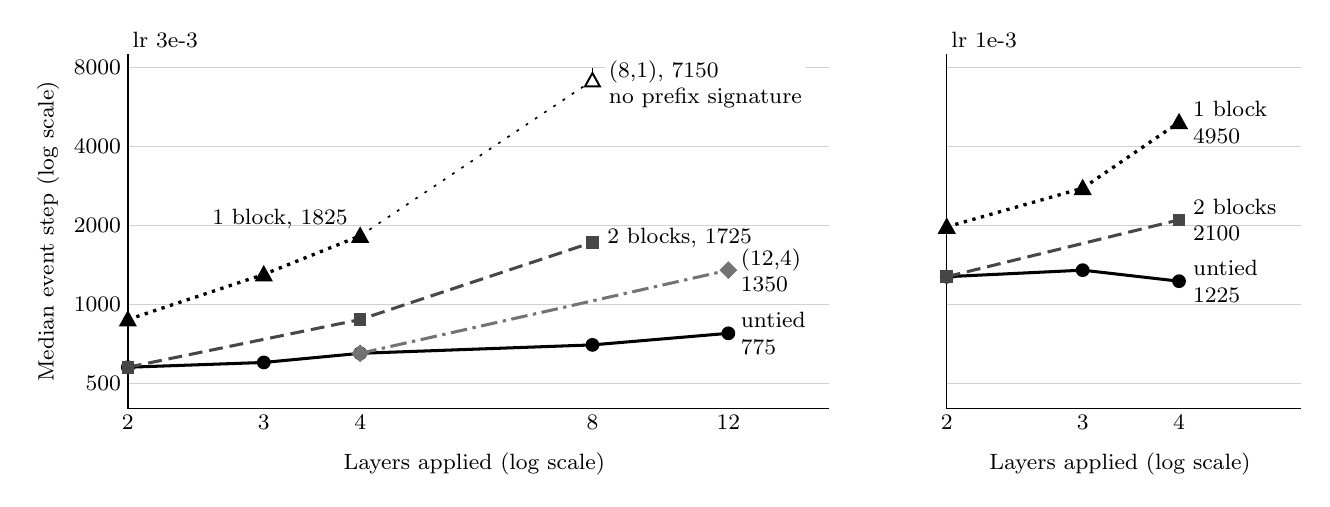
\begin{tikzpicture}
\draw[black!18, line width=0.4pt] (0.000,0.323) -- (8.900,0.323);
\draw[black!18, line width=0.4pt] (10.400,0.323) -- (14.900,0.323);
\node[anchor=east, inner sep=1.5pt, align=left, font=\footnotesize] at (-0.030,0.323) {500};
\draw[black!18, line width=0.4pt] (0.000,1.324) -- (8.900,1.324);
\draw[black!18, line width=0.4pt] (10.400,1.324) -- (14.900,1.324);
\node[anchor=east, inner sep=1.5pt, align=left, font=\footnotesize] at (-0.030,1.324) {1000};
\draw[black!18, line width=0.4pt] (0.000,2.326) -- (8.900,2.326);
\draw[black!18, line width=0.4pt] (10.400,2.326) -- (14.900,2.326);
\node[anchor=east, inner sep=1.5pt, align=left, font=\footnotesize] at (-0.030,2.326) {2000};
\draw[black!18, line width=0.4pt] (0.000,3.328) -- (8.900,3.328);
\draw[black!18, line width=0.4pt] (10.400,3.328) -- (14.900,3.328);
\node[anchor=east, inner sep=1.5pt, align=left, font=\footnotesize] at (-0.030,3.328) {4000};
\draw[black!18, line width=0.4pt] (0.000,4.330) -- (8.900,4.330);
\draw[black!18, line width=0.4pt] (10.400,4.330) -- (14.900,4.330);
\node[anchor=east, inner sep=1.5pt, align=left, font=\footnotesize] at (-0.030,4.330) {8000};
\draw[black, line width=0.5pt] (0.000,4.500) -- (0.000,0.000) -- (8.900,0.000);
\draw[black, line width=0.5pt] (10.400,4.500) -- (10.400,0.000) -- (14.900,0.000);
\node[anchor=north, inner sep=1.5pt, align=left, font=\footnotesize] at (0.000,-0.030) {2};
\node[anchor=north, inner sep=1.5pt, align=left, font=\footnotesize] at (1.726,-0.030) {3};
\node[anchor=north, inner sep=1.5pt, align=left, font=\footnotesize] at (2.950,-0.030) {4};
\node[anchor=north, inner sep=1.5pt, align=left, font=\footnotesize] at (5.900,-0.030) {8};
\node[anchor=north, inner sep=1.5pt, align=left, font=\footnotesize] at (7.626,-0.030) {12};
\node[anchor=north, inner sep=1.5pt, align=left, font=\footnotesize] at (10.400,-0.030) {2};
\node[anchor=north, inner sep=1.5pt, align=left, font=\footnotesize] at (12.126,-0.030) {3};
\node[anchor=north, inner sep=1.5pt, align=left, font=\footnotesize] at (13.350,-0.030) {4};
\node[anchor=north, inner sep=1.5pt, align=left, font=\footnotesize] at (4.400,-0.500) {Layers applied (log scale)};
\node[anchor=north, inner sep=1.5pt, align=left, font=\footnotesize] at (12.600,-0.500) {Layers applied (log scale)};
\node[anchor=south west, inner sep=1.5pt, align=left, font=\footnotesize] at (0.000,4.530) {lr 3e-3};
\node[anchor=south west, inner sep=1.5pt, align=left, font=\footnotesize] at (10.400,4.530) {lr 1e-3};
\node[rotate=90, anchor=south, font=\footnotesize] at (-0.75,2.250) {Median event step (log scale)};
\draw[black, line width=1.1pt] (0.000,0.525) -- (1.726,0.586) -- (2.950,0.702) -- (5.900,0.809) -- (7.626,0.956);
\draw[black, line width=0.5pt] (0.000,0.525) -- (0.000,0.525);
\draw[black, fill=black, line width=0.7pt] (0.000,0.525) circle (0.075);
\draw[black, line width=0.5pt] (1.726,0.586) -- (1.726,0.645);
\draw[black, fill=black, line width=0.7pt] (1.726,0.586) circle (0.075);
\draw[black, line width=0.5pt] (2.950,0.702) -- (2.950,0.702);
\draw[black, fill=black, line width=0.7pt] (2.950,0.702) circle (0.075);
\draw[black, line width=0.5pt] (5.900,0.809) -- (5.900,0.860);
\draw[black, fill=black, line width=0.7pt] (5.900,0.809) circle (0.075);
\draw[black, line width=0.5pt] (7.626,0.909) -- (7.626,1.002);
\draw[black, fill=black, line width=0.7pt] (7.626,0.956) circle (0.075);
\draw[black!72, line width=1.1pt, dash pattern=on 5pt off 2.5pt] (0.000,0.525) -- (2.950,1.131) -- (5.900,2.112);
\draw[black!72, line width=0.5pt] (0.000,0.525) -- (0.000,0.525);
\draw[black!72, fill=black!72, line width=0.7pt] (-0.068,0.457) rectangle (0.068,0.593);
\draw[black!72, line width=0.5pt] (2.950,1.089) -- (2.950,1.131);
\draw[black!72, fill=black!72, line width=0.7pt] (2.882,1.063) rectangle (3.018,1.199);
\draw[black!72, line width=0.5pt] (5.900,2.048) -- (5.900,2.112);
\draw[black!72, fill=black!72, line width=0.7pt] (5.832,2.044) rectangle (5.968,2.180);
\draw[black, line width=1.2pt, dash pattern=on 1.2pt off 2pt] (0.000,1.131) -- (1.726,1.704) -- (2.950,2.194);
\draw[black, line width=0.5pt] (0.000,1.131) -- (0.000,1.172);
\draw[black, fill=black, line width=0.7pt] (0.000,1.226) -- (-0.095,1.055) -- (0.095,1.055) -- cycle;
\draw[black, line width=0.5pt] (1.726,1.618) -- (1.726,1.731);
\draw[black, fill=black, line width=0.7pt] (1.726,1.799) -- (1.631,1.628) -- (1.821,1.628) -- cycle;
\draw[black, line width=0.5pt] (2.950,2.133) -- (2.950,2.271);
\draw[black, fill=black, line width=0.7pt] (2.950,2.289) -- (2.855,2.118) -- (3.045,2.118) -- cycle;
\draw[black!55, line width=1.1pt, dash pattern=on 6pt off 2pt on 1.2pt off 2pt] (2.950,0.702) -- (7.626,1.758);
\draw[black!55, line width=0.5pt] (2.950,0.702) -- (2.950,0.702);
\draw[black!55, fill=black!55, line width=0.7pt] (2.950,0.797) -- (2.855,0.702) -- (2.950,0.607) -- (3.045,0.702) -- cycle;
\draw[black!55, line width=0.5pt] (7.626,1.704) -- (7.626,1.811);
\draw[black!55, fill=black!55, line width=0.7pt] (7.626,1.853) -- (7.531,1.758) -- (7.626,1.663) -- (7.721,1.758) -- cycle;
\draw[black, line width=0.6pt, dash pattern=on 1pt off 3pt] (2.950,2.194) -- (5.900,4.167);
\draw[black, line width=0.5pt] (5.900,4.095) -- (5.900,4.330);
\draw[black, fill=white, line width=0.7pt] (5.900,4.262) -- (5.805,4.091) -- (5.995,4.091) -- cycle;
\node[anchor=west, inner sep=1.5pt, align=left, font=\footnotesize] at (7.726,0.956) {untied\\775};
\node[anchor=west, inner sep=1.5pt, align=left, font=\footnotesize] at (6.030,2.172) {2 blocks, 1725};
\node[anchor=east, inner sep=1.5pt, align=left, font=\footnotesize] at (2.850,2.414) {1 block, 1825};
\node[anchor=west, inner sep=1.5pt, align=left, font=\footnotesize, fill=white] at (6.050,4.117) {(8,1), 7150\\no prefix signature};
\node[anchor=west, inner sep=1.5pt, align=left, font=\footnotesize] at (7.726,1.758) {(12,4)\\1350};
\draw[black, line width=1.1pt] (10.400,1.675) -- (12.126,1.758) -- (13.350,1.618);
\draw[black, line width=0.5pt] (10.400,1.647) -- (10.400,1.704);
\draw[black, fill=black, line width=0.7pt] (10.400,1.675) circle (0.075);
\draw[black, line width=0.5pt] (12.126,1.731) -- (12.126,1.759);
\draw[black, fill=black, line width=0.7pt] (12.126,1.758) circle (0.075);
\draw[black, line width=0.5pt] (13.350,1.588) -- (13.350,1.647);
\draw[black, fill=black, line width=0.7pt] (13.350,1.618) circle (0.075);
\draw[black!72, line width=1.1pt, dash pattern=on 5pt off 2.5pt] (10.400,1.675) -- (13.350,2.397);
\draw[black!72, line width=0.5pt] (10.400,1.647) -- (10.400,1.704);
\draw[black!72, fill=black!72, line width=0.7pt] (10.332,1.607) rectangle (10.468,1.743);
\draw[black!72, line width=0.5pt] (13.350,2.362) -- (13.350,2.414);
\draw[black!72, fill=black!72, line width=0.7pt] (13.282,2.329) rectangle (13.418,2.465);
\draw[black, line width=1.2pt, dash pattern=on 1.2pt off 2pt] (10.400,2.308) -- (12.126,2.799) -- (13.350,3.636);
\draw[black, line width=0.5pt] (10.400,2.271) -- (10.400,2.326);
\draw[black, fill=black, line width=0.7pt] (10.400,2.403) -- (10.305,2.232) -- (10.495,2.232) -- cycle;
\draw[black, line width=0.5pt] (12.126,2.773) -- (12.126,2.863);
\draw[black, fill=black, line width=0.7pt] (12.126,2.894) -- (12.031,2.723) -- (12.221,2.723) -- cycle;
\draw[black, line width=0.5pt] (13.350,3.606) -- (13.350,3.700);
\draw[black, fill=black, line width=0.7pt] (13.350,3.731) -- (13.255,3.560) -- (13.445,3.560) -- cycle;
\node[anchor=west, inner sep=1.5pt, align=left, font=\footnotesize] at (13.470,1.618) {untied\\1225};
\node[anchor=west, inner sep=1.5pt, align=left, font=\footnotesize] at (13.470,2.397) {2 blocks\\2100};
\node[anchor=west, inner sep=1.5pt, align=left, font=\footnotesize] at (13.470,3.636) {1 block\\4950};
\end{tikzpicture}
